\documentclass[12pt]{article}
\usepackage[utf8]{inputenc}
\usepackage[T1]{fontenc}
\usepackage{graphicx,amsmath,amsfonts,amssymb,float,caption,geometry,hyperref,url,booktabs,listings,xcolor}
\geometry{a4paper,margin=2.5cm}
\graphicspath{{figuras/}}
\lstset{basicstyle=\ttfamily\scriptsize,breaklines=true,numbers=left,numberstyle=\tiny,frame=single,keywordstyle=\color{blue},commentstyle=\color{gray}}
\newcommand{\ms}{\,\mathrm{ms}}
\newcommand{\mV}{\,\mathrm{mV}}
\newcommand{\Hz}{\,\mathrm{Hz}}
\newcommand{\gu}{\,\mathrm{mS/cm^2}}
\newcommand{\Ju}{\,\mu\mathrm{A/cm^2}}

\title{Lista 8: Introduction to Computational Neuroscience}
\author{Pierina Milla}
\date{October 2026}

\begin{document}
\maketitle

%=====================================================================
\section*{Models and numerical methods}

All simulations use three single-compartment Hodgkin--Huxley-type neurons: an excitatory pyramidal cell (E, Olufsen et al.), a fast-spiking basket interneuron (I, Wang--Buzs\'aki) and an oriens-lacunosum-moleculare interneuron (O, Tort et al.), with the equations given in the problem statement. The synaptic current is
\[
J_{\mathrm{sin},ij}(t)=\bar g_{ij}\,s_i(t)\,\bigl(E_{\mathrm{rev}}-V_j(t)\bigr),
\qquad
\frac{ds}{dt}=\frac{1+\tanh(V_{\mathrm{pre}}/4)}{2}\,\frac{1-s}{\tau_s}-\frac{s}{\tau_d},
\]
where $i$ is the presynaptic and $j$ the postsynaptic neuron. The sign of $J_{\mathrm{sin}}$ is set by the driving force $E_{\mathrm{rev}}-V_j$: AMPA synapses ($E_{\mathrm{rev}}=0\mV$) depolarize and GABA$_\mathrm{A}$ synapses ($E_{\mathrm{rev}}=-80\mV$) hyperpolarize the postsynaptic cell, because $V_j$ always lies between these values.

The equations were integrated with the fourth-order Runge--Kutta method and $\Delta t=0.01\ms$. A spike is registered at each upward crossing of $0\mV$, and its time is obtained by linear interpolation inside the time step. The Fortran program, the shell script that runs all cases and the Python plotting script are listed in the appendices. Random initial voltages (uniform in $[-70,-60]\mV$) use a fixed seed, so every number below is reproducible; the effect of other seeds was not tested. As a check on the O-neuron equations, the initial values prescribed in the statement ($m=0.0122$, $n=0.0756$, $a=0.0229$ at $V=-75.61\mV$) coincide with the stationary values $m_\infty$, $n_\infty$, $a_\infty$ computed from Eqs.~(15), (17) and (18).

%=====================================================================
\section*{Question 1: Synaptic interaction between two neurons}

This question investigates how a presynaptic neuron affects a postsynaptic neuron through a unidirectional synapse. In all items the neurons start at $V(0)=-65\mV$ with $h$ and $n$ at their stationary values, and the external current is applied only to the presynaptic neuron. For (a) and (b) the pulse lasts from $t=5\ms$ to $t=15\ms$.

\subsection*{(a) Excitatory-to-inhibitory connection}

The presynaptic neuron is E, the postsynaptic neuron is I, and $\bar g_{EI}=0.05\gu$. The simulation lasts $30\ms$. Since the statement only asks for \emph{a} value of $J_0$ giving a single presynaptic spike, a scan of $J_0$ was performed (file \texttt{data/q1\_varreduras.txt}): $J_0=0.2$ and $0.4\Ju$ produce no spike, every tested value from $0.6$ to $3.8\Ju$ produces exactly one E spike, and $J_0=4$ and $5\Ju$ produce two. The value $J_0=3\Ju$ is used in Figure~\ref{fig:q1a}.

\begin{figure}[H]
\centering
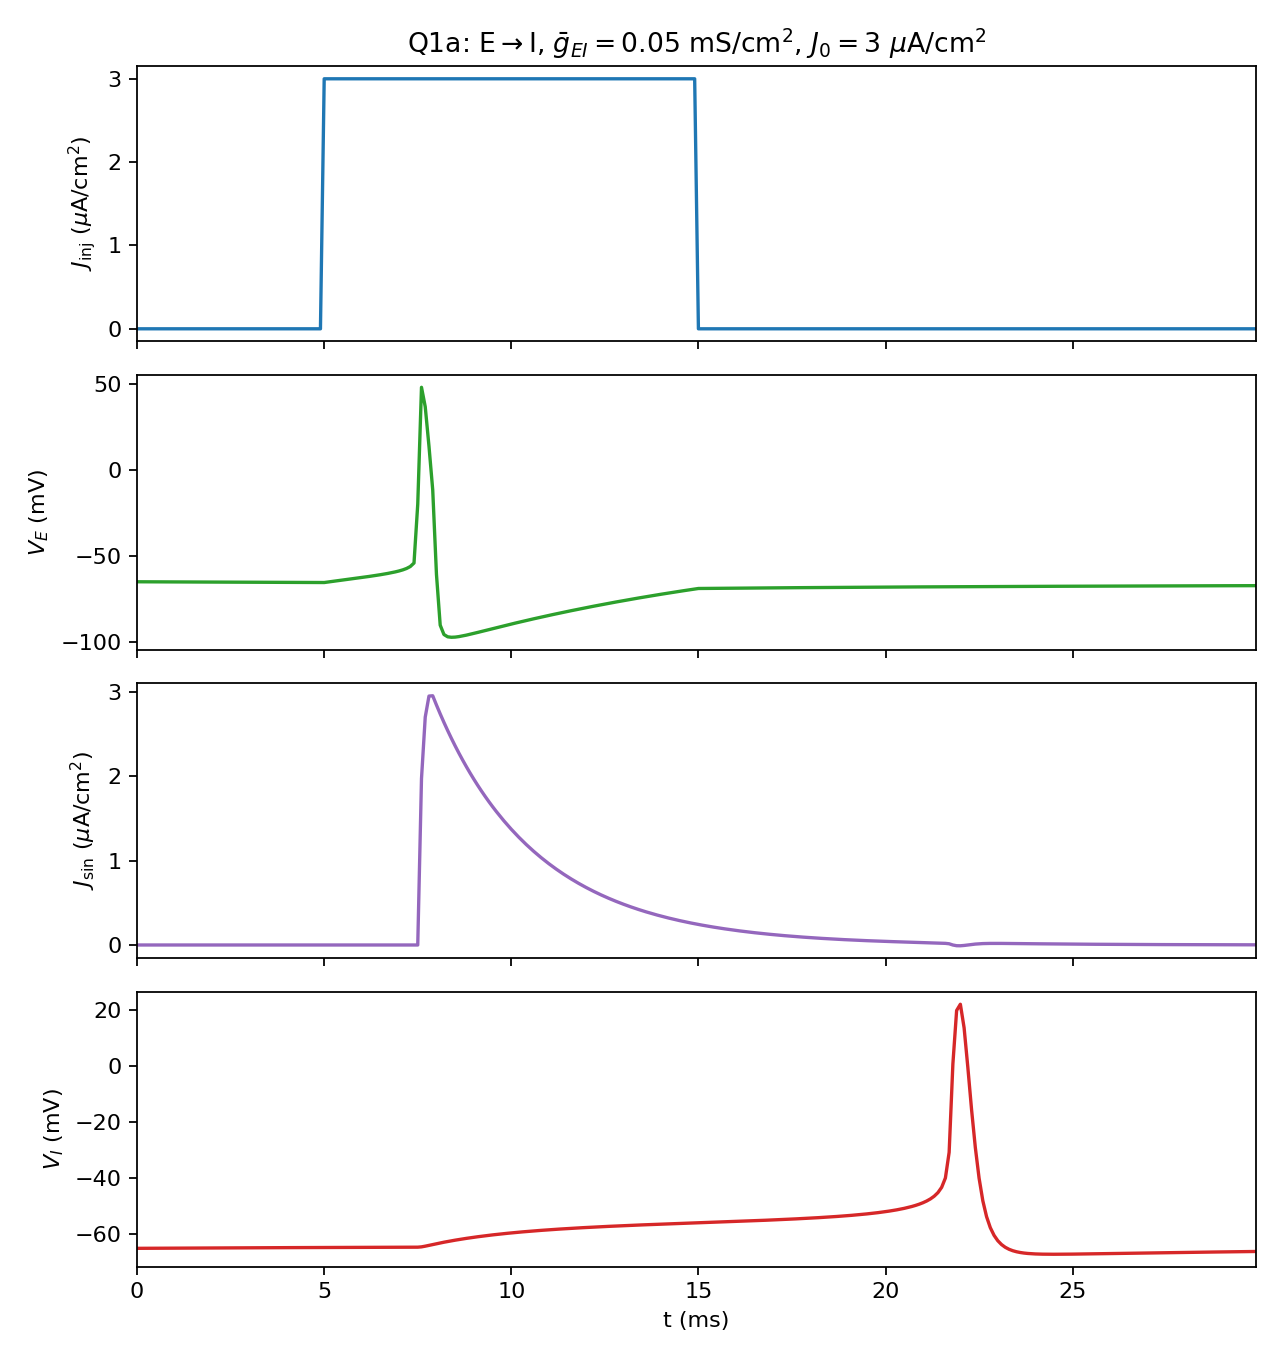
\includegraphics[width=0.92\textwidth]{Q1a_E_to_I.png}
\caption{Question 1(a): E$\to$I connection with $\bar g_{EI}=0.05\gu$ and $J_0=3\Ju$. From top to bottom: applied current, presynaptic voltage $V_E$, synaptic current $J_{\mathrm{sin}}$, and postsynaptic voltage $V_I$.}
\label{fig:q1a}
\end{figure}

The E neuron emits one spike at $t=7.5\ms$. The synaptic variable $s$ rises with the fast time constant $\tau_s=0.1\ms$ (peak $s\simeq0.93$) and decays with $\tau_d=3\ms$, so $J_{\mathrm{sin}}$ is a brief, positive (depolarizing) pulse with peak $\simeq2.95\Ju$. The I neuron responds with one spike at $t=21.8\ms$, i.e.\ $14.3\ms$ after the presynaptic spike. The postsynaptic spike is therefore not immediate: the brief AMPA current only brings $V_I$ to threshold after a latency, and the long latency is consistent with the Wang--Buzs\'aki cell being an excitable neuron that can fire at arbitrarily low rates near threshold. After the spike $V_I$ undershoots to $-67.1\mV$ and relaxes back towards rest.

\subsection*{(b) Inhibitory-to-excitatory connection}

The roles are exchanged: I is presynaptic and receives the pulse, E is postsynaptic, and $\bar g_{IE}=0.1\gu$. The simulation was extended to $100\ms$. The scan shows that the I neuron needs a different current than the E neuron: $J_0=0.5\Ju$ gives no spike, $J_0=1$, $1.5$ and $2\Ju$ give exactly one, and $J_0=3$ and $4\Ju$ give two. A current of $4\Ju$ therefore does \emph{not} satisfy the one-spike requirement (two I spikes occur, at $8.6\ms$ and $14.8\ms$), whereas $J_0=2\Ju$ does and is used in Figure~\ref{fig:q1b}.

\begin{figure}[H]
\centering
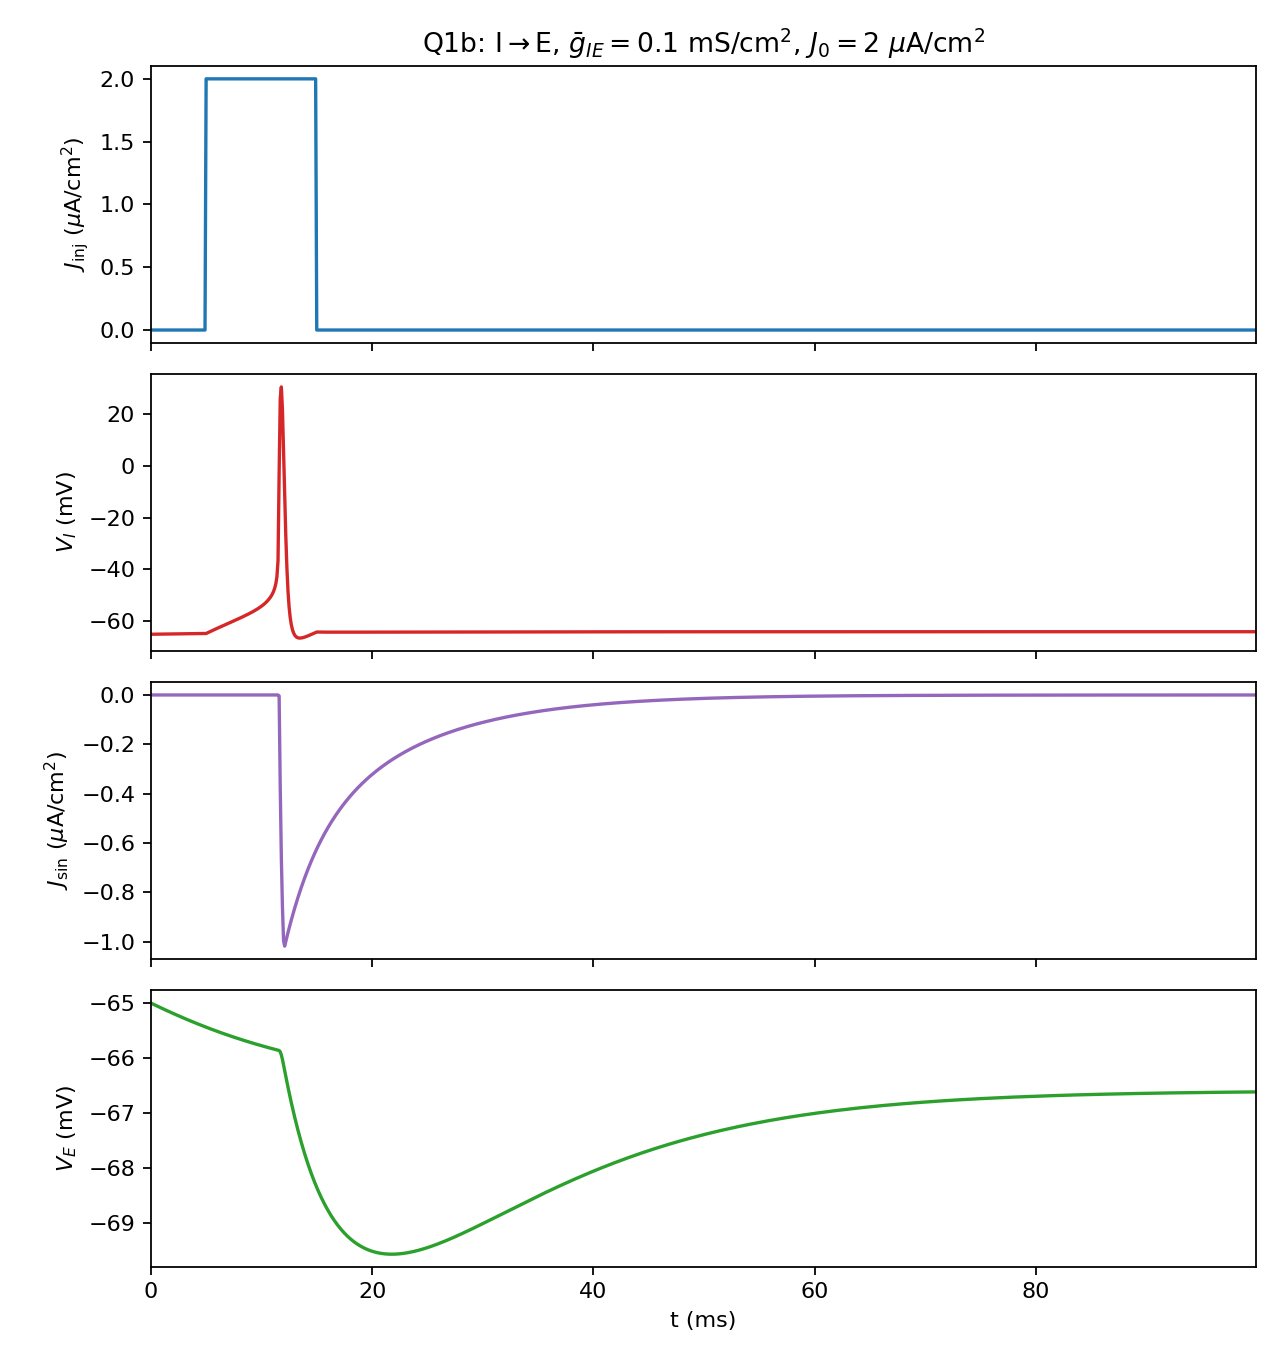
\includegraphics[width=0.92\textwidth]{Q1b_I_to_E.png}
\caption{Question 1(b): I$\to$E connection with $\bar g_{IE}=0.1\gu$ and $J_0=2\Ju$. From top to bottom: applied current, presynaptic voltage $V_I$, synaptic current $J_{\mathrm{sin}}$, and postsynaptic voltage $V_E$.}
\label{fig:q1b}
\end{figure}

The I neuron fires once, at $t=11.6\ms$. Because $E_{\mathrm{rev}}=-80\mV<V_E$, the synaptic current is negative, with peak magnitude $\simeq1.02\Ju$. The E neuron does not fire; its voltage, which relaxes towards a resting value of about $-66.6\mV$, is pushed down to a minimum of $-69.6\mV$ at $t=21.8\ms$ (an inhibitory postsynaptic potential of roughly $3\mV$) and then recovers. Within the $100\ms$ window no postsynaptic spike appears. The effect of the synapse is thus opposite in sign to that of item (a).

\subsection*{(c) Repetitive firing and the effect of $\bar g_{EI}$}

The E neuron receives a current step of $J_0=1.5\Ju$ from $t=5\ms$ to $t=450\ms$ (simulation of $500\ms$) and drives the I neuron. The E neuron fires regularly, 26 spikes in total, with interspike interval
\[
T=17.66\ms\qquad\Longrightarrow\qquad f_E=\frac{1}{T}\simeq 56.6\Hz .
\]
(The last interval is longer, $17.95\ms$, because the current is switched off at $450\ms$.) The period does not depend on $\bar g_{EI}$, since there is no feedback from I to E in this configuration.

The I neuron emits a spike train for \emph{all ten} conductances $\bar g_{EI}=0.10,0.12,\dots,0.28\gu$ (Table~\ref{tab:q1d}). Supplementary runs below the requested range show that the response begins between $0.01$ and $0.02\gu$ (no I spike at $0.01$; $4$, $9$, $13$, $16$, $22$ and $26$ spikes at $0.02$, $0.03$, $0.04$, $0.05$, $0.06$ and $0.08\gu$), so $0.10\gu$ already lies in the regime where each E spike evokes an I spike. Figure~\ref{fig:q1c} shows the voltages.

\begin{figure}[H]
\centering
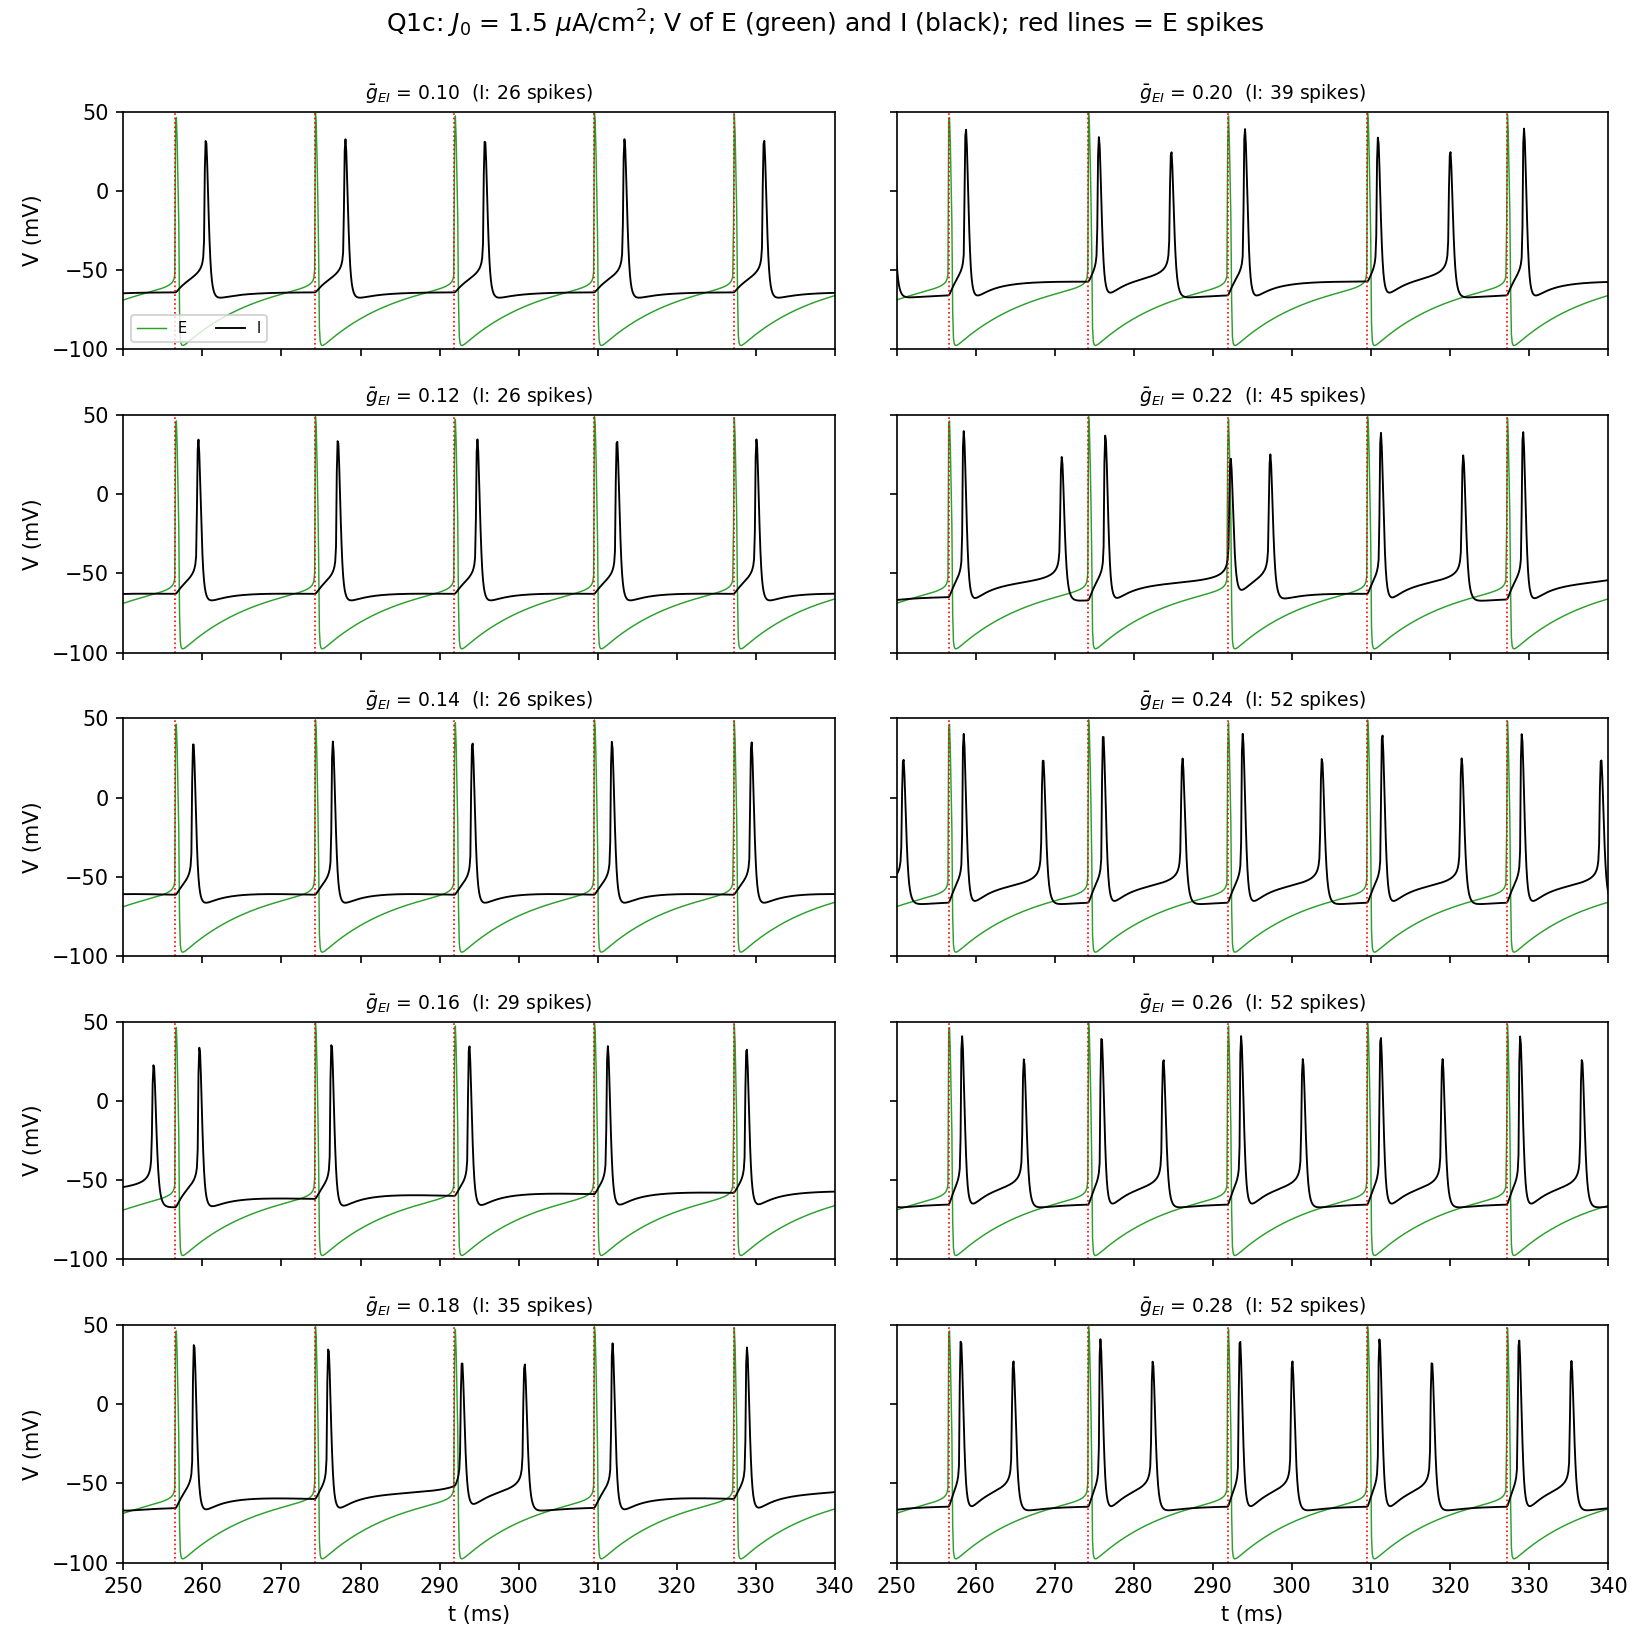
\includegraphics[width=\textwidth]{Q1c_sweep.png}
\caption{Question 1(c): voltages of the E (green) and I (black) neurons for the ten values of $\bar g_{EI}$, in a window of $90\ms$ taken during the steady firing. The red dotted lines mark the E spikes. For $0.10$--$0.14\gu$ the I neuron fires once per E spike; for larger $\bar g_{EI}$ extra I spikes appear between successive E spikes.}
\label{fig:q1c}
\end{figure}

\subsection*{(d) Entrainment and phase locking}

\emph{Entrainment} means that the postsynaptic firing frequency equals (or is a simple multiple of) the presynaptic one; \emph{phase locking} means that the delay $\delta$ between the presynaptic spike and the postsynaptic spike(s) is constant from cycle to cycle. For every E spike, $\delta$ was measured as the time from that spike to each I spike that follows it before the next E spike (Figure~\ref{fig:q1d}). A regime was classified as phase-locked only when the pattern of I spikes repeats every $m$ E cycles with spike times matching within $0.15\ms$ over the last $14$ repetitions of the window $100$--$445\ms$. This criterion is deliberately strict, and the window contains only about $18$ cycles, so a regime labelled ``no strict locking'' may be a slow transient or quasi-periodic rather than truly irregular.

\begin{figure}[H]
\centering
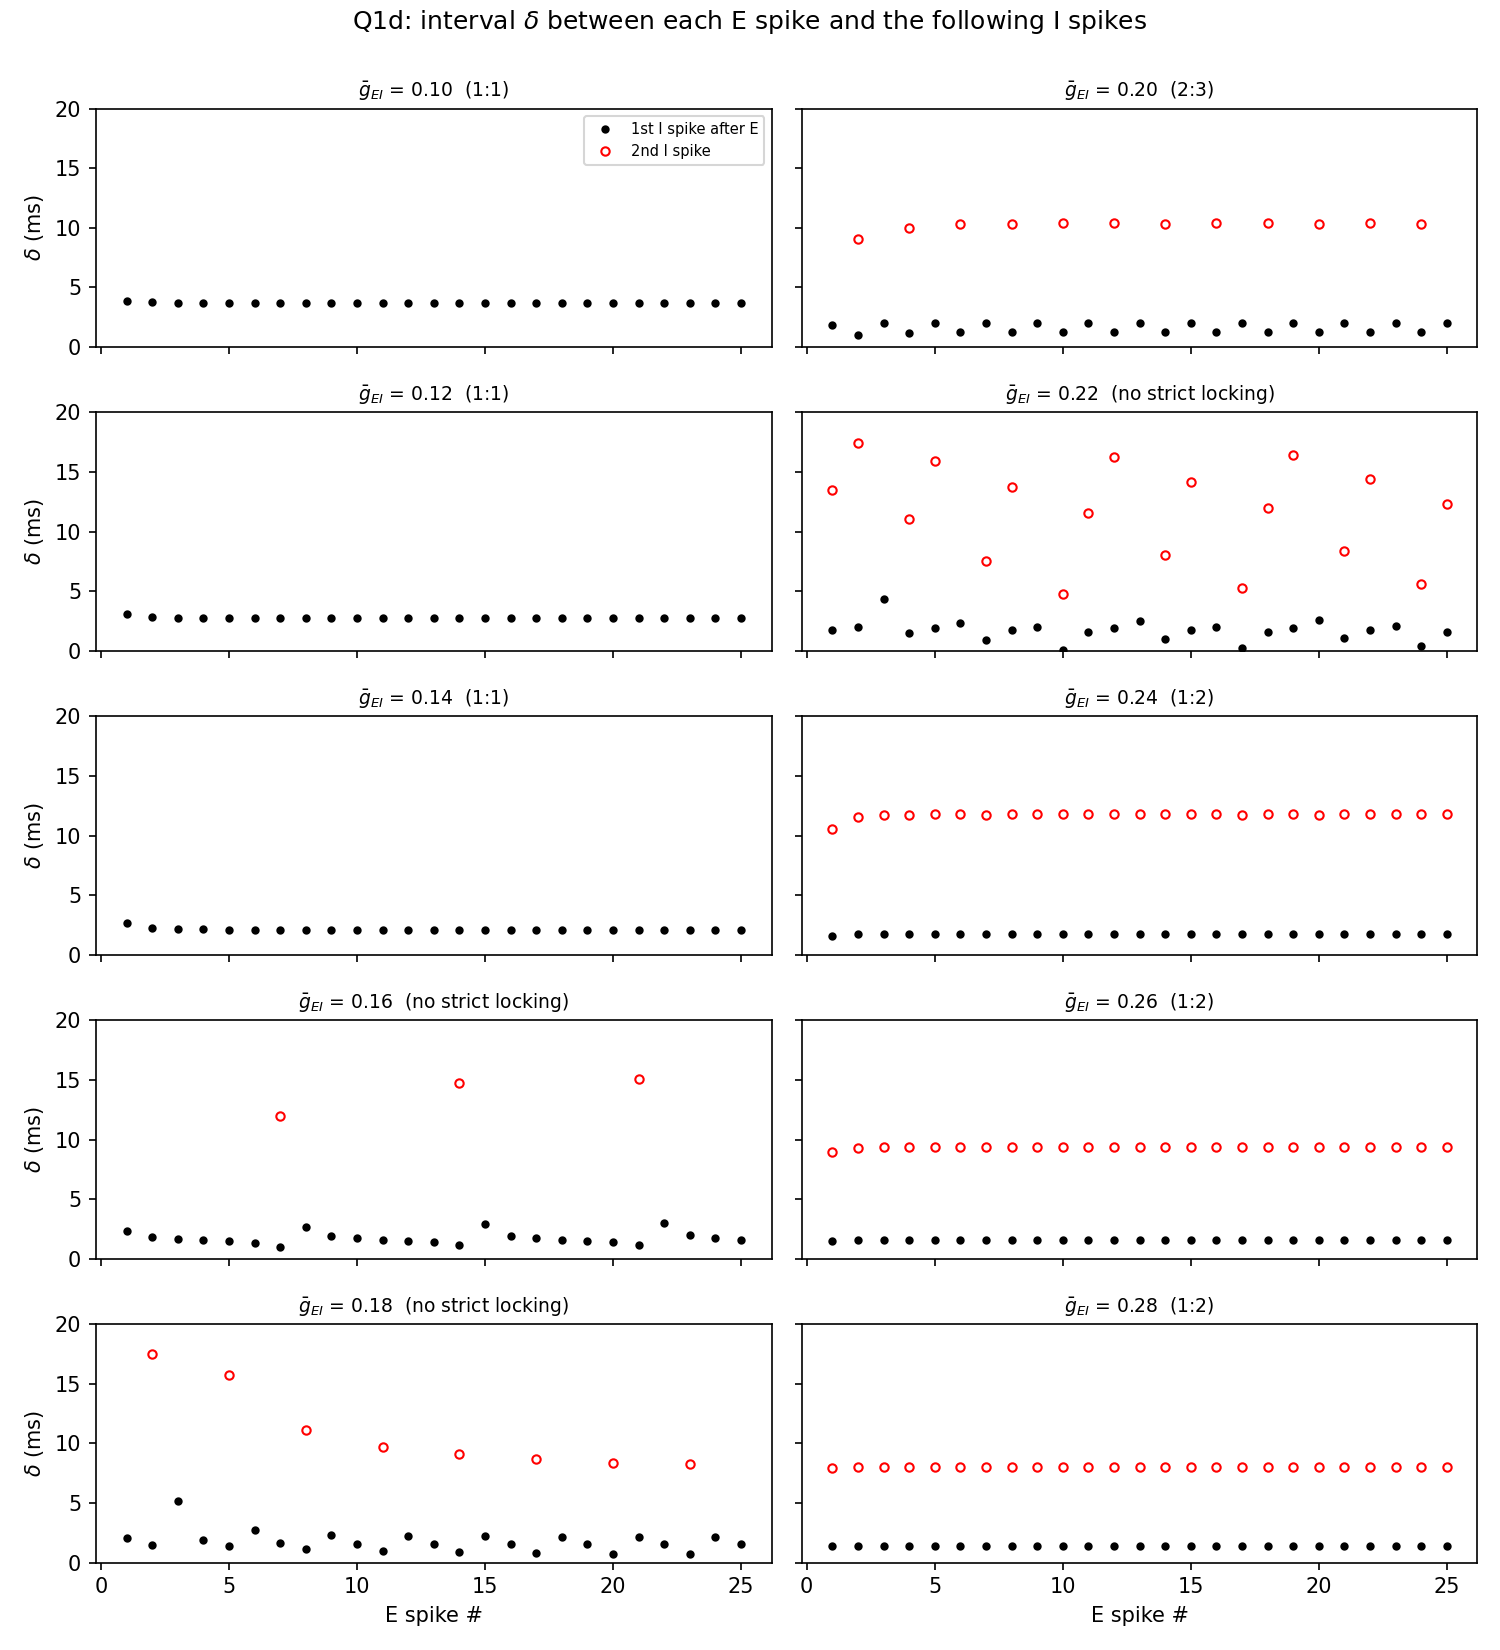
\includegraphics[width=0.92\textwidth]{Q1d_delta.png}
\caption{Question 1(d): interval $\delta$ between each E spike and the I spikes that follow it, for the ten values of $\bar g_{EI}$ (black: first I spike after the E spike; red circles: second I spike in the same cycle). Titles give the locking ratio (E spikes : I spikes).}
\label{fig:q1d}
\end{figure}

\begin{figure}[H]
\centering
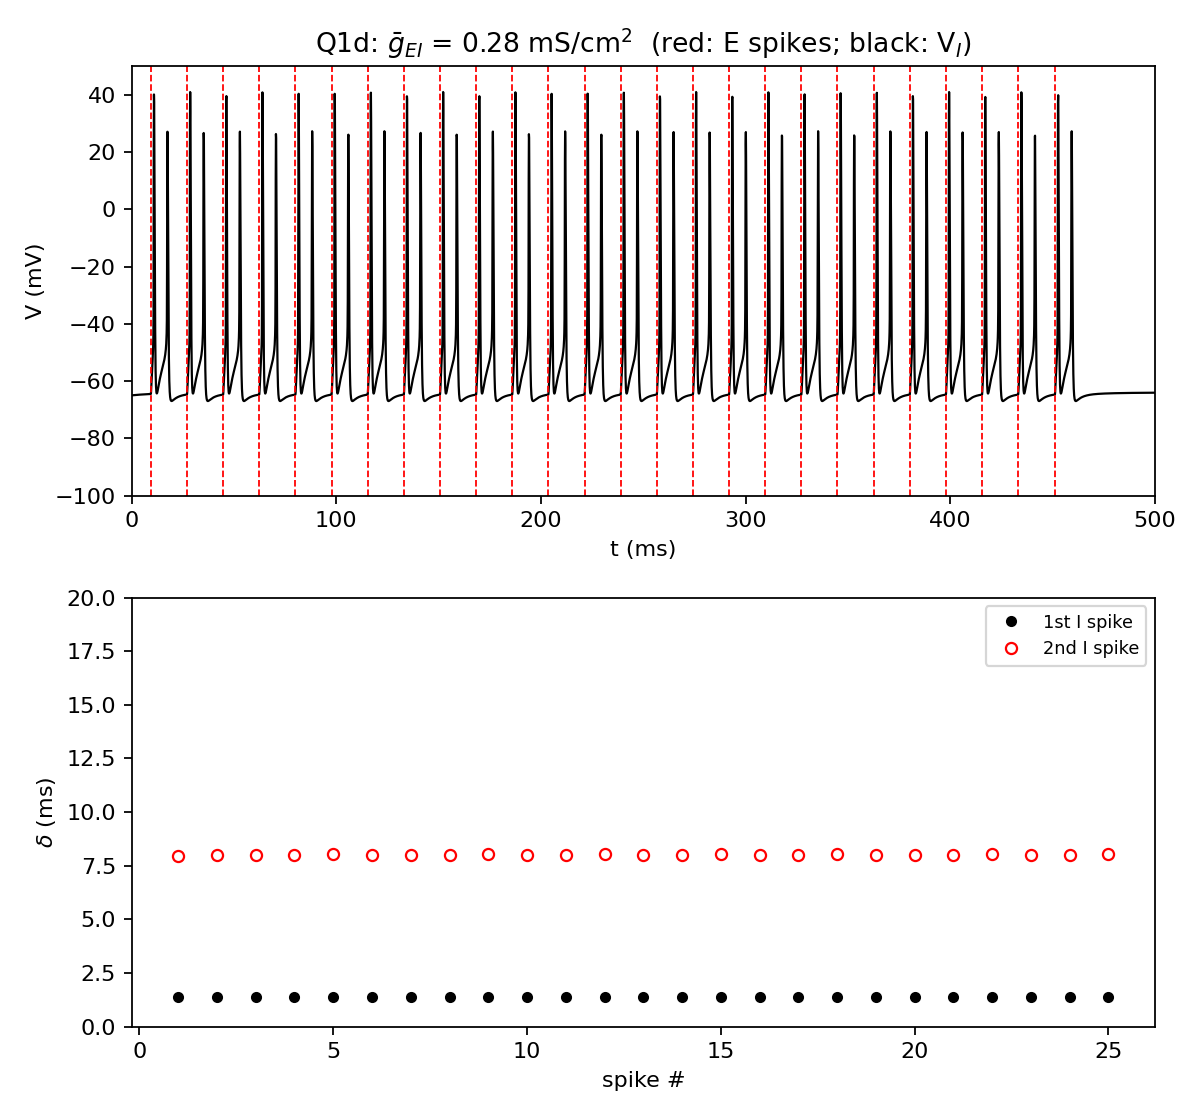
\includegraphics[width=0.7\textwidth]{Q1d_g_0.28.png}
\caption{Question 1(d), example in the format of Figure~3 of the statement ($\bar g_{EI}=0.28\gu$). Top: $V_I$ (black) with the E spike times (red dashed lines). Bottom: $\delta$ for each E spike (black: first I spike, red circles: second).}
\label{fig:q1d28}
\end{figure}

\begin{table}[H]
\centering
\begin{tabular}{cccp{0.40\textwidth}}
\toprule
$\bar g_{EI}$ ($\mathrm{mS/cm^2}$) & I spikes (E: 26) & E:I locking & $\delta$ (ms)\\
\midrule
0.10 & 26 & 1:1 & 3.69\\
0.12 & 26 & 1:1 & 2.74\\
0.14 & 26 & 1:1 & 2.10\\
0.16 & 29 & no strict locking & mostly one I spike per cycle with an occasional extra spike\\
0.18 & 35 & no strict locking & extra I spike every third cycle, but its $\delta$ drifts from $\simeq17$ to $\simeq8\ms$\\
0.20 & 39 & 2:3 & first spike alternates between $\simeq1.2$ and $\simeq2.0$; second spike at $\simeq10.3$\\
0.22 & 45 & no strict locking & irregular pattern of one or two I spikes per cycle\\
0.24 & 52 & 1:2 & 1.75 and 11.8\\
0.26 & 52 & 1:2 & 1.55 and 9.36\\
0.28 & 52 & 1:2 & 1.40 and 8.02\\
\bottomrule
\end{tabular}
\caption{Question 1(d): firing pattern of the I neuron for each $\bar g_{EI}$ ($J_0=1.5\Ju$).}
\label{tab:q1d}
\end{table}

\paragraph{Answer.} Frequency entrainment with phase locking in the $1{:}1$ sense (one postsynaptic spike per presynaptic spike, constant $\delta$) occurs for $\bar g_{EI}=0.10$, $0.12$ and $0.14\gu$. In the notation of the statement, ``$n{:}1$'' entrainment ($n\ge2$ presynaptic spikes per postsynaptic spike) was \emph{not} observed for any $\bar g_{EI}$, because the I neuron never skips an E spike; for larger $\bar g_{EI}$ it instead fires \emph{more} often than E. In E:I terms, locked regimes with two I spikes per E spike ($1{:}2$, for $0.24$, $0.26$ and $0.28\gu$) and with three I spikes per two E spikes ($2{:}3$, for $0.20\gu$) were found. For $\bar g_{EI}=0.16$, $0.18$ and $0.22\gu$ no strict locking was detected in $450\ms$. In the $1{:}2$ cases the two intervals between I spikes sum to the E period (e.g.\ $11.04+6.62=17.66\ms=T$ for $0.28\gu$), as expected for locking.

\subsection*{Summary of Question 1}

\begin{table}[H]
\centering
\begin{tabular}{p{0.08\textwidth}p{0.36\textwidth}p{0.46\textwidth}}
\toprule
\textbf{Item} & \textbf{Parameters} & \textbf{Result}\\
\midrule
(a) & E$\to$I, $\bar g_{EI}=0.05$, $J_0=3\Ju$ & E spike at $7.5\ms$; I spike at $21.8\ms$ (latency $14.3\ms$). Any $J_0$ from $0.6$ to $3.8\Ju$ (tested values) gives one E spike.\\
(b) & I$\to$E, $\bar g_{IE}=0.1$, $J_0=2\Ju$ & One I spike at $11.6\ms$; E is inhibited ($V_E^{\min}=-69.6\mV$), no E spike. $J_0=4\Ju$ gives two I spikes and does not qualify.\\
(c) & $J_0=1.5\Ju$ step, ten values of $\bar g_{EI}$ & $T=17.66\ms$ ($56.6\Hz$). The I neuron fires a train for all ten values.\\
(d) & same & $1{:}1$ locking for $0.10$--$0.14\gu$; $2{:}3$ for $0.20$; $1{:}2$ for $0.24$--$0.28$; no strict locking for $0.16$, $0.18$, $0.22$. No $n{:}1$ with $n\ge2$.\\
\bottomrule
\end{tabular}
\caption{Summary of Question 1.}
\label{tab:q1summary}
\end{table}

%=====================================================================
\section*{Question 2: Rhythms generated by an inhibitory network (ING)}

The network has five I and five O neurons: every O projects to every I ($\bar g_{OI}=0.04\gu$), every I projects to every O ($\bar g_{IO}=0.12\gu$) and every I projects to every I, including itself ($\bar g_{II}=0.02\gu$); there are no O--O connections. All I neurons receive $J=1\Ju$ and all O neurons $J=-3\Ju$. The O neurons start from the values given in the statement, and the initial $V$ of each I neuron is drawn uniformly from $[-70,-60]\mV$ with $h$ and $n$ at their stationary values. The simulation lasts $1500\ms$. Frequencies and the synchrony index below were computed for $t>500\ms$. The index is $\chi=\sigma_{\bar V}/\langle\sigma_{V_i}\rangle_i$, the standard deviation (in time) of the population-mean voltage divided by the mean of the individual standard deviations; $\chi=1$ means perfect synchrony.

\subsection*{(a) ING network with O$\to$I synapses}

\begin{figure}[H]
\centering
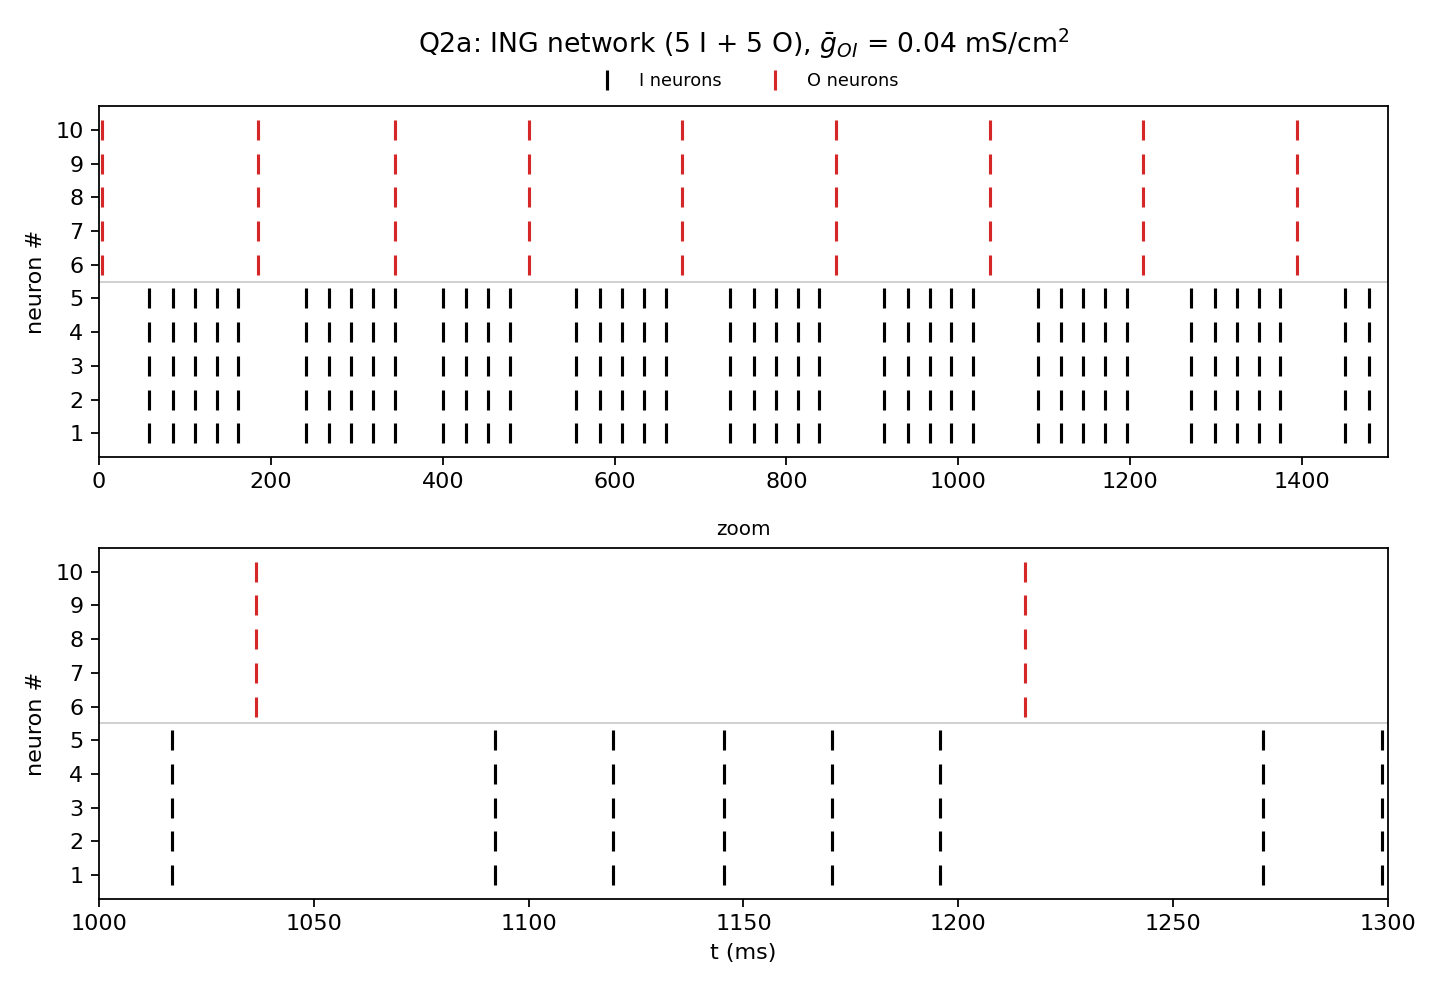
\includegraphics[width=0.95\textwidth]{Q2a_raster.png}
\caption{Question 2(a): raster plot of the network with $\bar g_{OI}=0.04\gu$ (neurons 1--5: I, black; neurons 6--10: O, red). Top: $1500\ms$. Bottom: zoom on $1000$--$1300\ms$.}
\label{fig:q2a}
\end{figure}

The I neurons fire in bursts of gamma-frequency spikes (interspike interval $\simeq25\ms$, i.e.\ $\simeq39\Hz$), separated by silent gaps of $\simeq75\ms$ instead of $25\ms$: an O volley arrives about $20\ms$ after the last I spike of a burst and postpones the next I spike (in the cycles inspected, for example at $500$, $679$ and $858\ms$); their mean rate is $27\Hz$. The O neurons fire in volleys at a rate of $\simeq5.6\Hz$ (interval $178.9\ms$), in the theta band. The five I neurons converge to identical spike times (they are already coincident from the first I spike, at $58.6\ms$) and the five O neurons are synchronous from the start ($\chi=1.00$ for both populations). The O neurons are synchronous trivially, since they have identical initial conditions and inputs. The I neurons synchronize because they receive a common, strong inhibitory input from the first O volley at $2.9\ms$ and because of their mutual inhibition. So the network shows convergence to synchronous firing, with a gamma rhythm in I nested in a theta rhythm set by O. The O neurons fire repeatedly despite the negative injected current; this is presumably due to rebound from their $h$- and $A$-type currents, but that mechanism was not tested here.

\subsection*{(b) Without O$\to$I synapses}

\begin{figure}[H]
\centering
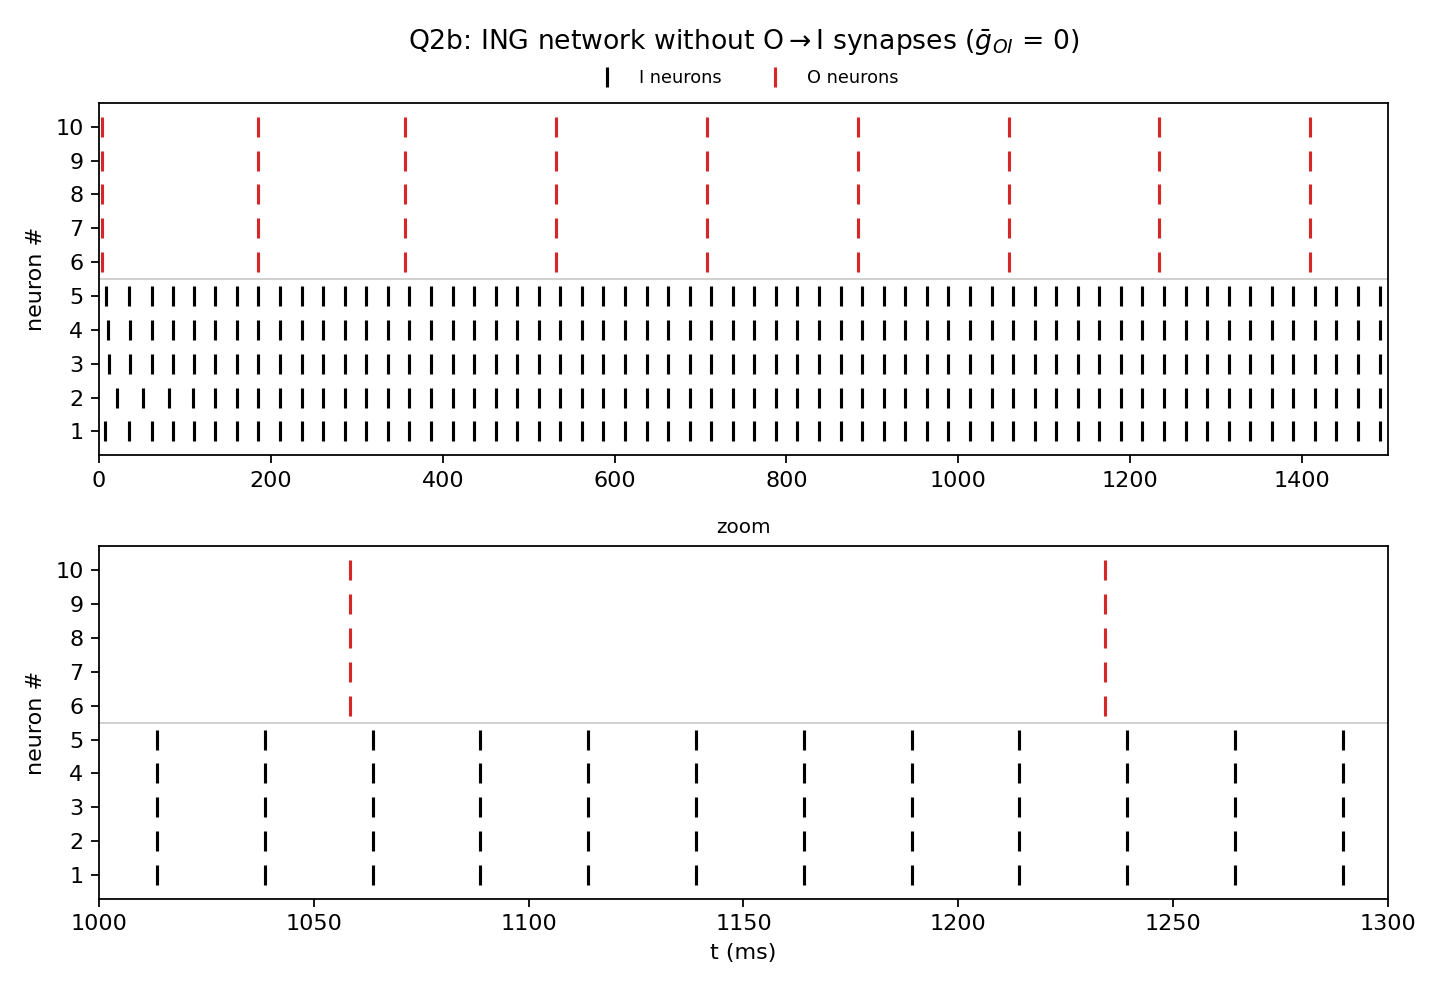
\includegraphics[width=0.95\textwidth]{Q2b_raster.png}
\caption{Question 2(b): raster plot with $\bar g_{OI}=0$.}
\label{fig:q2b}
\end{figure}

Without the O$\to$I synapses the I population becomes a pure ING oscillator: all I neurons fire with a constant interval of $25.1\ms$ ($39.9\Hz$, mean rate $40\Hz$), with no gaps (299 I spikes versus 205 in item (a)). The I neurons start with different phases (their first spikes lie between $7.5$ and $20.6\ms$) and converge to a synchronous rhythm ($\chi=1.00$ for $t>500\ms$). The O neurons still fire at the theta rate ($5.7\Hz$, interval $175.6\ms$), now under an uninterrupted gamma-frequency inhibition from I. The main difference from (a) is thus the absence of the theta-timed pauses in the I population: the O$\to$I synapses are what interrupts the gamma rhythm of I once per O cycle.

\subsection*{Summary of Question 2}

\begin{table}[H]
\centering
\begin{tabular}{p{0.08\textwidth}p{0.20\textwidth}p{0.30\textwidth}p{0.28\textwidth}}
\toprule
\textbf{Item} & \textbf{Condition} & \textbf{I neurons} & \textbf{O neurons}\\
\midrule
(a) & $\bar g_{OI}=0.04$ & gamma bursts (ISI $\simeq25\ms$, $\simeq39\Hz$) with $\simeq75\ms$ pauses; mean rate $27\Hz$; synchronous & $5.6\Hz$ (theta); synchronous\\
(b) & $\bar g_{OI}=0$ & continuous gamma, ISI $25.1\ms$ ($39.9\Hz$); synchronous & $5.7\Hz$\\
\bottomrule
\end{tabular}
\caption{Summary of Question 2 ($t>500\ms$).}
\label{tab:q2summary}
\end{table}

%=====================================================================
\section*{Question 3: Rhythms in networks of excitatory and inhibitory neurons (PING)}

\subsection*{(a) Minimal PING network}

One E neuron and one I neuron are connected E$\to$I and I$\to$E (no autapses), with $\bar g_{EI}=\bar g_{IE}=0.25\gu$, $J_E=1.4\Ju$ and $J_I=0$. The statement does not give initial conditions for this item, so both neurons start at $V=-65\mV$ with $h$ and $n$ stationary. The simulation lasts $200\ms$.

\begin{figure}[H]
\centering
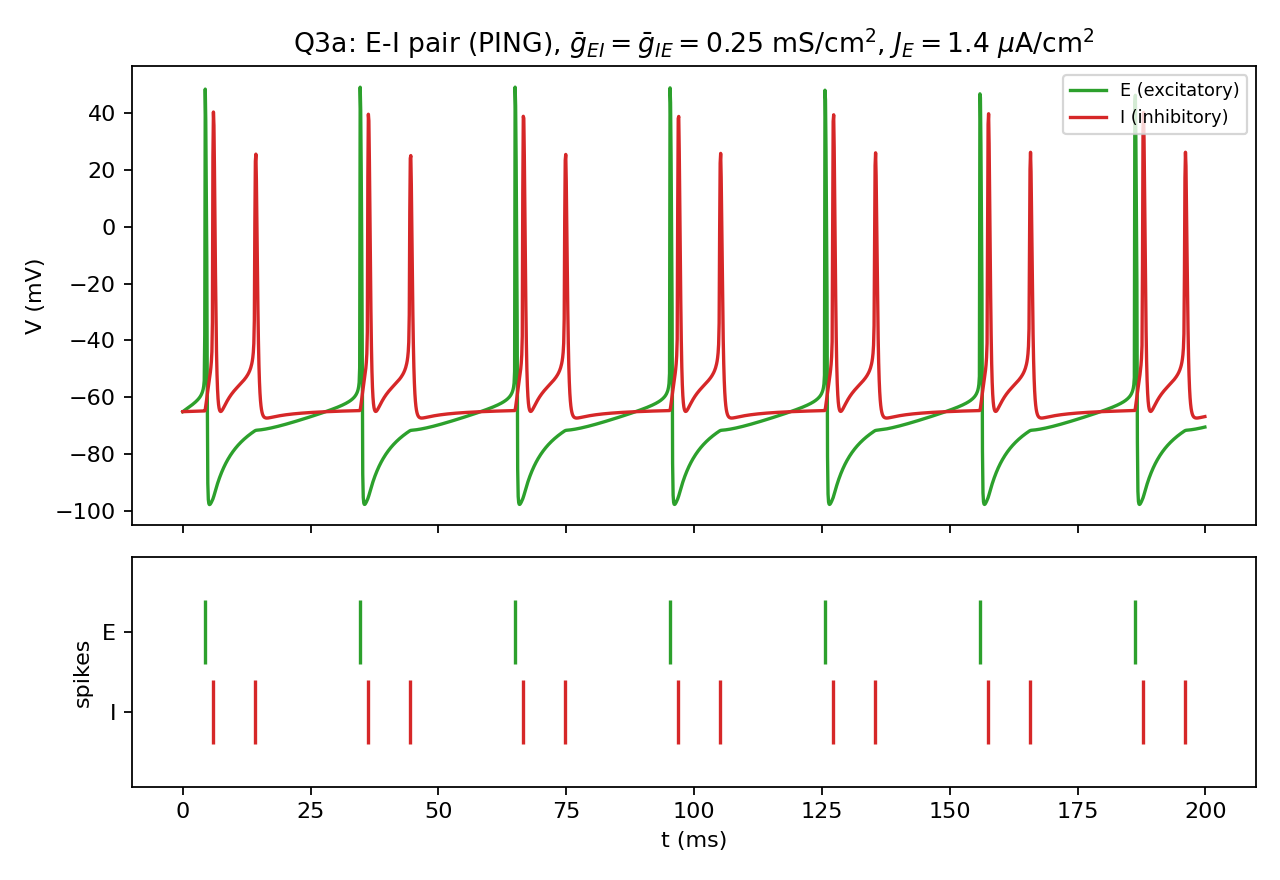
\includegraphics[width=0.92\textwidth]{Q3a_VEI.png}
\caption{Question 3(a): voltages of the E (green) and I (red) neurons, with the corresponding spike times in the lower panel.}
\label{fig:q3a}
\end{figure}

The two neurons oscillate periodically with $T=30.3\ms$ ($33\Hz$, in the gamma band). In each cycle the E neuron fires first and the I neuron fires \emph{twice}: the first I spike occurs $\simeq1.5\ms$ after the E spike and the second one $\simeq9.8\ms$ after it. The sequence is E, I, I, E, I, I, \dots The mechanism is the one that gives PING its name: the E spike activates I through AMPA, I fires and the resulting GABA$_\mathrm{A}$ current silences E (note the hyperpolarization to $\simeq-97\mV$ after each E spike); E recovers when the inhibition decays and fires again. The double I spike is a property of this parameter set: the residual AMPA current from the E spike is strong enough ($\bar g_{EI}=0.25\gu$) to bring I back to threshold while E is still silenced.

\subsection*{(b) Sensitivity of the period}

The period $T$ was measured from the E spike times between $t=300$ and $1000\ms$ (simulations of $1000\ms$ instead of $200\ms$, to have enough cycles after the transient). The baseline is $T_0=30.310\ms$ (standard deviation of the intervals $0.008\ms$), which agrees with the value from the $200\ms$ run. Each parameter was perturbed by $1\%$ and the sensitivity $S_p\simeq(\Delta T/T)/(\Delta p/p)\approx \partial\ln T/\partial\ln p$ was computed with a one-sided difference.

\begin{figure}[H]
\centering
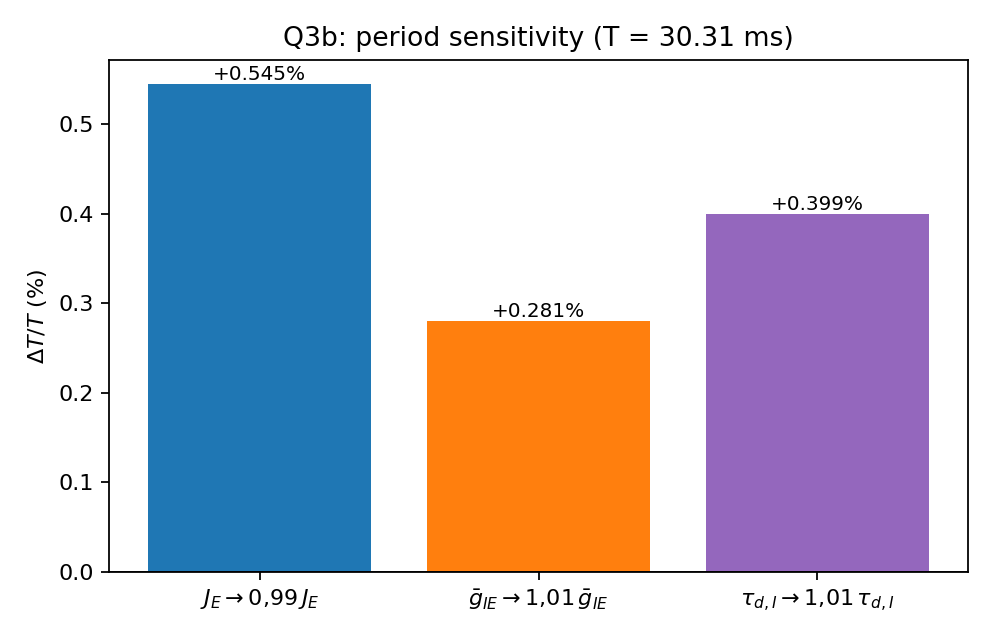
\includegraphics[width=0.6\textwidth]{Q3b_sensibilidade.png}
\caption{Question 3(b): percentage change of the period for each $1\%$ perturbation.}
\label{fig:q3b}
\end{figure}

\begin{table}[H]
\centering
\begin{tabular}{lccc}
\toprule
\textbf{Perturbation} & $T$ (ms) & $\Delta T/T$ (\%) & $S_p$\\
\midrule
baseline & 30.310 & --- & ---\\
$J_E\to0.99\,J_E$ & 30.475 & $+0.545$ & $-0.545$\\
$\bar g_{IE}\to1.01\,\bar g_{IE}$ & 30.395 & $+0.281$ & $+0.281$\\
$\tau_{d,I}\to1.01\,\tau_{d,I}$ & 30.431 & $+0.399$ & $+0.399$\\
\bottomrule
\end{tabular}
\caption{Question 3(b): period of the E--I oscillation under $1\%$ parameter changes.}
\label{tab:q3b}
\end{table}

The period is most sensitive to the current applied to the excitatory neuron, $J_E$: a $1\%$ decrease lengthens $T$ by $0.545\%$, which is about $1.4$ times the effect of $\tau_{d,I}$ and about $1.9$ times that of $\bar g_{IE}$. The signs are consistent with the mechanism: weaker drive to E, stronger inhibition or slower decay of the inhibition all delay the recovery of E and increase $T$. All changes are well above the cycle-to-cycle scatter of $0.008\ms$ in $T$, but they come from single-sided differences of $1\%$ in one parameter around one operating point, so the ranking should not be extrapolated to large changes.

\subsection*{(c) E neuron added to the ING network}

A single E neuron is added to the network of Question 2(a). It projects to all I and O neurons and receives synapses from all of them, with $\bar g_{IE}=0.1$, $\bar g_{OE}=0.15$, $\bar g_{EI}=0.05$, $\bar g_{EO}=0.01$, $\bar g_{OI}=0.2$, $\bar g_{IO}=0.5$ and $\bar g_{II}=0.1\gu$. The injected currents are $J_E=0.8$, $J_I=0.8$ and $J_O=-3\Ju$. The E neuron is initialized like the I neurons.

\begin{figure}[H]
\centering
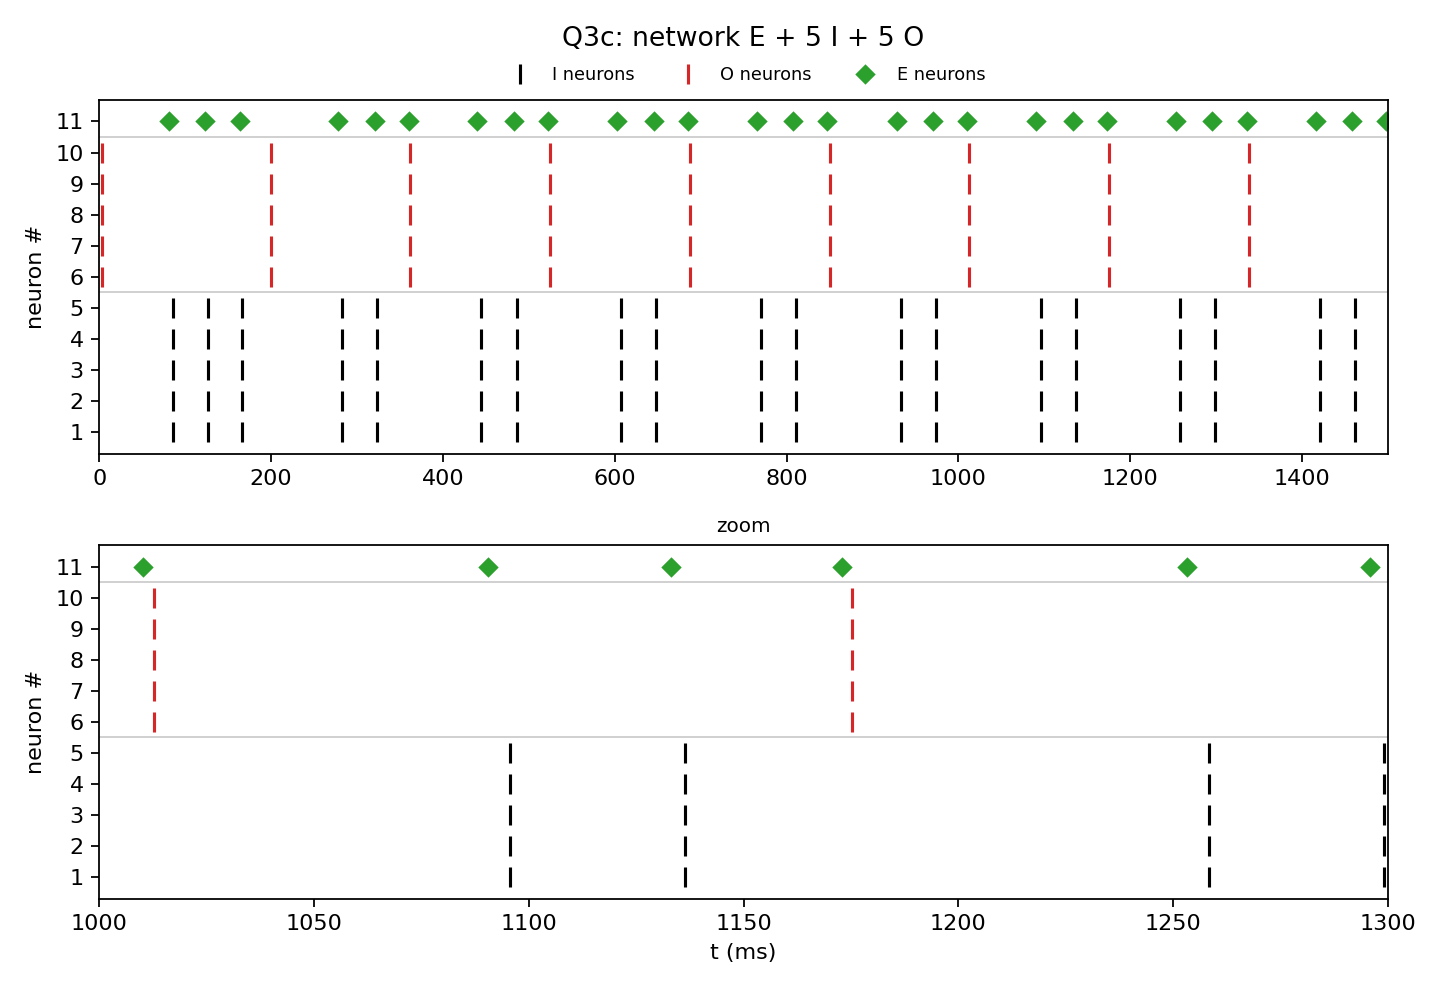
\includegraphics[width=0.95\textwidth]{Q3c_raster.png}
\caption{Question 3(c): raster plot of the network with one E neuron (green diamonds, top), five O neurons (red) and five I neurons (black).}
\label{fig:q3c}
\end{figure}

The I neurons fire in short groups of two or three spikes with interspike interval $\simeq41\ms$ ($\simeq24\Hz$), and the groups are separated by pauses of about $120$--$160\ms$, so their mean rate over $t>500\ms$ is only $12\Hz$ (95 I spikes versus 205 in Question 2(a)). The E neuron fires in the same groups, with the E spike preceding the I spikes by $\simeq3$--$5\ms$ (for example E at $807.8\ms$ and I at $811.1\ms$; E at $928.0\ms$ and I at $933.0\ms$), which is the PING order. The O volleys, at $\simeq6\Hz$ (interval $162.6\ms$), fall inside the pauses of the I population. The E spike that occurs about $2.4\ms$ before an O volley (for example at $847.6\ms$, with the O volley at $850.0\ms$) is not followed by an I spike. The five I neurons are synchronous ($\chi=1.00$).

Compared with the inhibitory-only network, the rhythm of the I population is therefore slower and sparser, and the gamma-range activity now comes with E leading I. This comparison must be read with care: besides adding E, the parameters $\bar g_{II}$, $\bar g_{OI}$, $\bar g_{IO}$ and $J_I$ also differ from those of Question 2(a) ($0.1$ vs $0.02$, $0.2$ vs $0.04$, $0.5$ vs $0.12\gu$ and $0.8$ vs $1\Ju$), so the changes cannot be attributed to the E neuron alone; separating these effects would require additional simulations that were not run.

\subsection*{(d) Without O$\to$I synapses}

\begin{figure}[H]
\centering
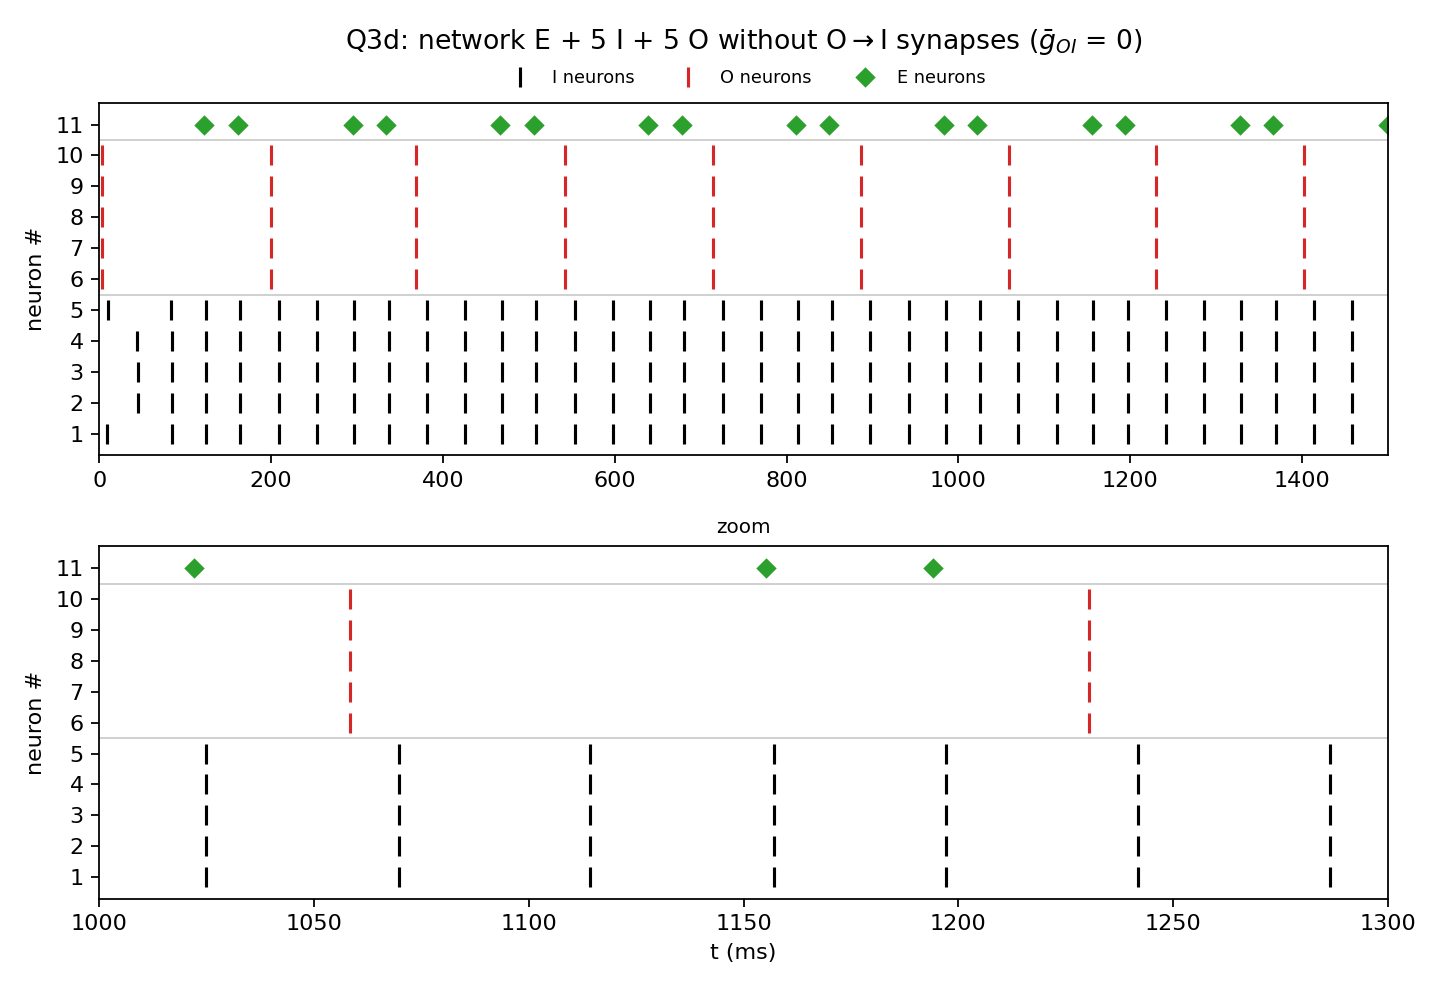
\includegraphics[width=0.95\textwidth]{Q3d_raster.png}
\caption{Question 3(d): raster plot of the network of item (c) with $\bar g_{OI}=0$.}
\label{fig:q3d}
\end{figure}

When the O$\to$I synapses are removed, the I neurons are no longer silenced by the O volleys and fire almost continuously with an interval of $\simeq44.6\ms$ ($\simeq22\Hz$; 170 I spikes against 95 in item (c)). The E neuron now fires in pairs of spikes ($\simeq40\ms$ apart), with one pair per O cycle: its pairs occur at $811$, $983$ and $1155\ms$, separated by $172\ms$, the period of the O neurons ($5.8\Hz$). The E neuron fires less often than in (c) (17 against 27 spikes in total). The I neurons remain synchronous ($\chi=1.00$). In short, without O$\to$I inhibition the E population fires one doublet per O cycle (it is locked to the O rhythm) instead of the I population being interrupted, as it does in item (c) and in Question 2(a).

\subsection*{Summary of Question 3}

\begin{table}[H]
\centering
\begin{tabular}{p{0.08\textwidth}p{0.88\textwidth}}
\toprule
\textbf{Item} & \textbf{Result}\\
\midrule
(a) & Order E, I, I per cycle; $T=30.3\ms$ ($33\Hz$). The first I spike follows E by $\simeq1.5\ms$, the second by $\simeq9.8\ms$.\\
(b) & $\Delta T/T$ for $1\%$ perturbations: $J_E$ ($-1\%$): $+0.545\%$; $\bar g_{IE}$ ($+1\%$): $+0.281\%$; $\tau_{d,I}$ ($+1\%$): $+0.399\%$. $T$ is most sensitive to $J_E$.\\
(c) & Groups of 2--3 spikes of E and I ($\simeq24\Hz$ within a group), E leading I by $3$--$5\ms$; O volleys at $\simeq6\Hz$ fall in the pauses; I mean rate $12\Hz$.\\
(d) & I fires almost continuously ($\simeq22\Hz$); E fires in doublets, one per O cycle ($172\ms$).\\
\bottomrule
\end{tabular}
\caption{Summary of Question 3.}
\label{tab:q3summary}
\end{table}

%=====================================================================
\section*{Conclusions}

The simulations illustrate three mechanisms by which synaptic coupling shapes neuronal activity. A single synapse changes the postsynaptic voltage with a sign set by $E_{\mathrm{rev}}-V$, and sustained presynaptic firing can lock the postsynaptic neuron in regimes that depend on $\bar g$ (Question 1). A purely inhibitory network of I and O neurons synchronizes into a gamma rhythm in I, interrupted at the theta rate of O when the O$\to$I synapses are present (Question 2). Adding an excitatory neuron produces the E-then-I ordering characteristic of PING, with a period that depends most strongly on the drive to E among the three parameters tested (Question 3). The statements about locking and about the networks of Question 3(c)--(d) are based on one realization of the random initial conditions and on windows of $450$--$1500\ms$.

%=====================================================================
\appendix
\section{Fortran code: \texttt{src/rede\_EIO.f90}}
\lstinputlisting[language={[90]Fortran}]{src/rede_EIO.f90}

\section{Shell script: \texttt{src/rodar\_tudo.sh}}
\lstinputlisting[language=bash]{src/rodar_tudo.sh}

\section{Python script: \texttt{src/graficos.py}}
\lstinputlisting[language=Python]{src/graficos.py}

\end{document}
